\documentclass[12pt]{article}
\usepackage{amsmath,amssymb,amsthm,amsopn}

\usepackage{graphicx}
\usepackage{tikz}
\usepackage{physics}

% adapted from Jelani Nelson's template

\DeclareMathOperator*{\E}{\mathbb{E}}
\let\Pr\relax
\DeclareMathOperator*{\Pr}{\mathbb{P}}

\newcommand{\eps}{\varepsilon}
\newcommand{\inprod}[1]{\left\langle #1 \right\rangle}
\newcommand{\R}{\mathbb{R}}
\newcommand{\C}{\mathbb{C}}
\newcommand{\T}{\mathbb{T}}
\newcommand{\Z}{\mathbb{Z}}
\newcommand{\N}{\mathbb{N}}

\newcommand{\handout}[5]{
  \noindent
  \begin{center}
  \framebox{
    \vbox{
      \hbox to 5.78in { {\bf MAT-280: Mathematical Foundations for Big Data } \hfill #2 }
      \vspace{4mm}
      \hbox to 5.78in { {\Large \hfill #5  \hfill} }
      \vspace{2mm}
      \hbox to 5.78in { {\em #3 \hfill #4} }
    }
  }
  \end{center}
  \vspace*{4mm}
}

\newcommand{\lecture}[4]{\handout{#1}{#2}{#3}{Scribes: #4}{Lecture #1}}

\newtheorem{theorem}{Theorem}
\newtheorem{corollary}[theorem]{Corollary}
\newtheorem{lemma}[theorem]{Lemma}
\newtheorem{proposition}[theorem]{Proposition}
\newtheorem{definition}[theorem]{Definition}
\newtheorem{assumption}[theorem]{Assumption}

\topmargin 0pt
\advance \topmargin by -\headheight
\advance \topmargin by -\headsep
\textheight 8.9in
\oddsidemargin 0pt
\evensidemargin \oddsidemargin
\marginparwidth 0.5in
\textwidth 6.5in

\parindent 0in
\parskip 1.5ex

\begin{document}

\lecture{1 --- April 1, 2016}{Spring 2016}{}{Sam Fleischer and Lily Silverstein}

\section{Probability Basics}

Expectation is denoted by $\E$.  Probability is denoted by $\Pr$.

The following two inequalities are independent of dimension.

\begin{theorem}[Markov's Inequality]
Let $X \geq 0$ be a random variable (RV) with $\E(X) < \infty$.  Then $$\Pr\qty(X > t) < \dfrac{\E(X)}{t}.$$
\end{theorem}

\begin{theorem}[Chebyshev's Inequality]
Let $X$ be a RV with $\E\qty(X^2) < \infty$.  Then $$\Pr\qty(\abs{X - \E(X)} > t) \leq \dfrac{\text{var}(X)}{t^2}.$$
\end{theorem}

\begin{proof}
  We apply Markov's Inequality to the RV $(X - \E(X))^2$ (which we know is $\geq 0$).  Then
  \begin{align*}
    \Pr\qty(\abs{X - \E(X)} > t) &= \Pr\qty((X - \E(X))^2 > t^2) \\
    &\leq \frac{\E\qty((X - \E(X))^2)}{t^2} \\
    &= \frac{\text{var}(X)}{t^2}
  \end{align*}
\end{proof}

The result of Markov's Inequality converges linearly to $0$ as $t \rightarrow \infty$, while the result of Chebyshev's Inequality converges quadratically to $0$.  Chebyshev's Inequality converges faster, but there is a tradeoff - we need knowledge of the variance of the RV $X$.  In big data applications, we often want to make statements about large subsets of the data.  The above inequalities are most useful when the bounds on the right hand side are close to $0$.

\subsection{Concentration Inequalities}

Concentration Inequalities can be thought of as ``blessings'' of high dimensionality. In big data applications we typically look at sums of many random variables $X_1, X_2, \dots, X_n$ as opposed to individual random variables.  We often ask the question ``How large is the sum $X_1 + X_2 + \dots + X_n$?''  We limit our discussion to independent and identically distributed (IID) random variables.

\begin{theorem}[Hoeffding's Inequality]
  Let $X_1, X_2, \dots, X_n$ be IID RVs with $\abs{X_i} \leq a$ and $\E(X_i) = 0$ for all $i$.  Then $$\Pr\qty(\abs{\sum_{i=1}^n X_i}>t) \leq 2\exp[\frac{-t^2}{2na^2}].$$
\end{theorem}

When $n$ is large, Hoeffding's Inequality shows there is little variance around the expected value.  In other words, the probability measure ``concentrates'' around $O(\sqrt{n})$.  More precisely,
\begin{align*}
  \abs{\sum_{i=1}^n X_i} \sim a\sqrt{n \log n}.
\end{align*}

For example, if $t = a\sqrt{2 n \log n}$, then by Hoeffding's Inequality,
\begin{align*}
  \Pr\qty(\abs{\sum_{i=1}^n X_i} > \sqrt{2 n \log n}) &\leq 2 \exp[\frac{- (a\sqrt{2 n \log n})^2}{2na^2}] \\
  &= 2 \exp[-\log n] \\
  &= \frac{2}{n}
\end{align*}
If $t = \dfrac{na}{2}$, the by Hoeffding's Inequality,
\begin{align*}
  \Pr\qty(\abs{\sum_{i=1}^n X_i} > \frac{na}{2}) &\leq 2 \exp[\frac{-\qty(\frac{na}{2})^2}{2na^2}] \\
  &= 2\exp[-\frac{n}{8}]
\end{align*}
Hoeffding's Inequality shows that choosing a larger $t$ gives greater confidence that the value will lie below $t$, whereas choosing a smaller $t$ gives the likelihood of highly concentrated data.  This is the tradeoff between high concentration and high probability.

\begin{theorem}[Bernstein's Inequality]
\end{theorem}

\begin{theorem}[Chernoff's Inequality]
\end{theorem}

\section{Spheres and Cubes in High Dimensions}

\subsection{Geometry of the $d$-dimensional Sphere}

Consider the unit sphere is $d$ dimensions.  Its volume is given by
\begin{align*}
  V(d) = \frac{\pi^{\frac{d}{2}}}{\frac{d}{2}\ \Gamma\qty(\frac{d}{2})}
\end{align*}
where $\Gamma$ is the Gamma function.  Recall that for positive integers $n$, $\Gamma(n) = (n - 1)!$.  Using Stirling's Formula,
\begin{align*}
  \Gamma(n) \sim \sqrt{\frac{2\pi}{n}}\qty(\frac{n}{e})^n
\end{align*}
we can see $\gamma\qty(\frac{d}{2})$ grows much faster than $\pi^{\frac{d}{2}}$, and hence
\begin{align*}
  V(d) \rightarrow 0 \qquad \text{as} \qquad d \rightarrow \infty.
\end{align*}
In words, the volume of the $d$-dimensional sphere with radius $1$ goes to $0$ as the dimension $d$ increases to infinity, i.e.~unit sphere in high dimensions have almost no volume (compare this to the unit cube, which always has volume $1$).

Also notice that ``most'' of the volume of the $d$-dimensional sphere is contained near the boundary of the sphere.  That is, for a $d$-dimensional sphere of radius $r$, most of the volume is contained in an annulus of width proportional to $\frac{r}{d}$.

\subsection{Geometry of the $d$-dimensional Cube}

Most of the volume of the high-dimensional cube is located in its corners.

\begin{proof}[Proof (probabilistic argument)]
  Pick a point at random in the box $[-1,1]^d$.  We want to calculate the probability that the point is also in the sphere.

  Let $x = \qty[x_1, \dots, x_d] \in \R^d$ and each $x_i \in [-1,1]$ chosed uniformly at random.  The event that $x$ also lies in the sphere means $$\norm{x}_2 = \sqrt{\sum_{i=1}^d x_i^2} \leq 1.$$  Let $z_i = x_i^2$ and note that
  \begin{align*}
    \E(z_i) = \frac{1}{2}\int_{-1}^1 t^2 \dd t = \frac{1}{3} \implies \E\qty(\norm{x}_2^2) = \frac{d}{3}
  \end{align*}
  and
  \begin{align*}
    \text{var}(z_i) = \frac{1}{2}\int_{-1}^1 t^4 \dd t - \qty(\frac{1}{3})^2 = \frac{1}{5} - \frac{1}{9} = \frac{4}{45} \leq \frac{1}{10}
  \end{align*}
  Using Chernoff's Inequality,
  \begin{align*}
    \Pr\qty(\norm{x}_2^2 \leq 1) &= \Pr\qty(\sum_{i=1}^d x_i^2 \leq 1) \\
    &= \Pr\qty(\sum_{i=1}^d \qty(z_i - \E(z_i)) \leq 1 - \frac{d}{3}) \\
    &\leq \exp[\frac{-(\frac{d}{3})^2}{\frac{4d}{10}}] \\
    &\leq \exp[-\frac{d}{4}].
  \end{align*}
  Since this value converges to $0$ as the dimension $d$ goes to infinity, this shows random points in high cubes are most likely outside the sphere.  In other words, almost all the volume of hypercubes lie in their corners.
\end{proof}

\subsection{Comparisons between the $d$-dimensional Sphere and Cube}

\begin{figure}[ht!]
  \centering
  \begin{tikzpicture}[scale=0.3]
  \draw (-5,5) -- (5,5) -- (5,-5) -- (-5,-5) -- (-5,5);
  \node[draw,circle,fill,scale=0.3] (origin) at (0,0) {};
  \draw[dashed] (0,0) -- node [left,midway] (half) { 0.5} (0,5);
  \draw[dashed] (0,0) -- node [right,midway] (root) {$\frac{\sqrt{2}}{2}$} (5,5);
  \draw[dashed] (0,0) -- node [above,near end] (one) {\qquad 1} (-10,0);
  \draw (0,0) circle (10);
  \end{tikzpicture}
  \caption{$2$-dimensional unit sphere and unit cube, centered at the origin.}
  \label{2dim}
\end{figure}

In two dimensions (Fig.~\ref{2dim}), the unit square is completely contained in the unit sphere.  The distance from the center to a vertex (radius of the circumscribed sphere) is $\frac{\sqrt{2}}{2}$ and the apothem (radius of the inscribed sphere) is $\frac{1}{2}$.  In four dimensions (Fig.~\ref{4dim}), the distance from the center to a vertex is $1$, so the vertices of the cube touch the surface of the sphere.  However, the apothem is still $\frac{1}{2}$.  The result, when projected in two dimensions no longer appears convex, however all hypercubes are convex.  This is part of the strangeness of higher dimensions - hypercubes are both convex and ``pointy.''  In dimensions greater than $4$ the distance from the center to a vertex is $\frac{\sqrt{d}}{2} > 1$, and thus the vertices of the hypercube extend far outside the sphere.

\begin{figure}[ht!]
  \centering
  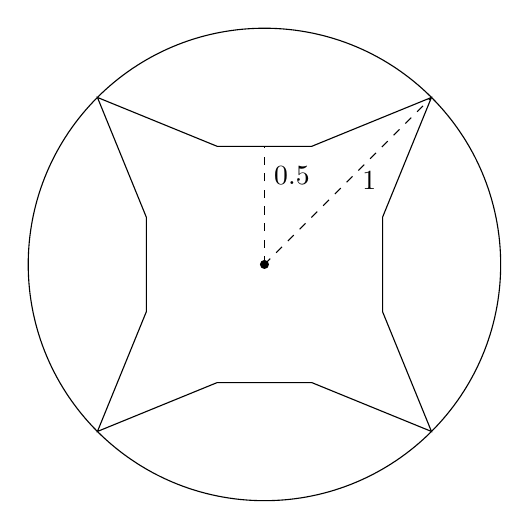
\begin{tikzpicture}[scale=0.3]
  \draw (2,5) -- (7.07,7.07) -- (5,2) -- ( 5,-2) -- (7.07,-7.07) -- (2,-5) -- (-2,-5) -- (-7.07,-7.07) -- (-5,-2) -- (-5,2) -- (-7.07,7.07) -- (-2,5) -- (2,5);
  \node[draw,circle,fill,scale=0.3] (origin) at (0,0) {};
  \draw[dashed] (0,0) -- node [right,near end] (half) {0.5} (0,5);
  \draw[dashed] (0,0) -- node [right,midway] (one) {\,1} (7.07,7.07);
  \draw (0,0) circle (10);
  \end{tikzpicture}
  \caption{Projections of the $4$-dimensional unit sphere and unit cube, centered at the origin.}
  \label{4dim}
\end{figure}

\section{Distances in High Dimensions}

\begin{theorem}[homework]
  Two random variables in high dimensions are almost orthogonal.
\end{theorem}

\subsection{Behavior of the $\ell^p$ norm in High Dimensions}

Assume we are given $n$ points $x^{(1)}, x^{(2)}, \dots, x^{(n)}$ in $\R^d$.  Define the $\ell^p$ norm of $x \in \R^d$ as
\begin{align*}
  \norm{x}_p = \qty(\sum_{i=1}^d \abs{x_i}^p)^{\frac{1}{p}}
\end{align*}
Define the \emph{relative contrast} of the data set as
\begin{align*}
  \frac{D_{\text{max}} - D_{\text{min}}}{D_{\text{min}}}
\end{align*}
where
\begin{align*}
  D_{\text{max}} &= \max_i \left\{\norm{x^{(i)}}_p\right\}, \qquad \text{and} \\
  D_{\text{min}} &= \min_i \left\{\norm{x^{(i)}}_p\right\}
\end{align*}
Relative contrast is useful in machine learning by identifying when a nearest-neighbor calculation is significant.

\end{document}
